\begin{frame}{Neural Network considered}
    \vspace{-2pt}
    We consider a parametric NN with 4 inputs and 4 outputs, defined by
    $$U_\theta(\bm{x},\bm{\mu}) = \big(u_\theta,v_\theta,p_\theta,T_\theta)(\bm{x},\bm{\mu}).$$
    
    The Dirichlet boundary conditions are imposed on the outputs of the MLP by a \textbf{post-processing} step. \citep{Sukumar_2022}
    
    \begin{center}
        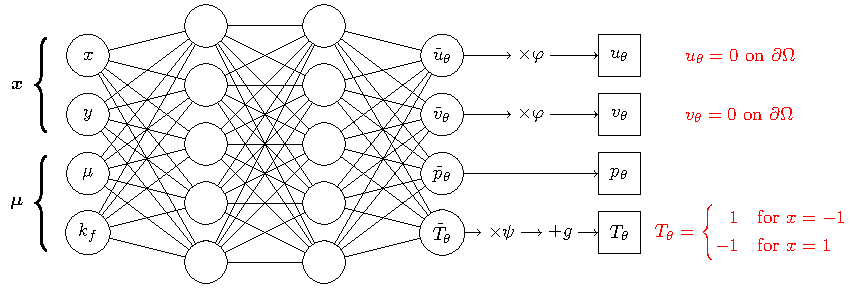
\includegraphics[width=0.74\linewidth]{images/pinn/network/network.pdf}
    \end{center}
    We consider two levelsets functions $\varphi$ and $\psi$, and the linear function $g$ defined by
    \begin{equation*}
        \varphi(x,y) = (x-1)(x+1)(y-1)(y+1),
    \end{equation*}
    \begin{equation*}
        \psi(x,y) = (x-1)(x+1) \quad \text{and} \quad g(x,y) = 1 - (x+1).
    \end{equation*}
\end{frame}

\begin{frame}{PINN losses}
    \textbf{Approximation of the solution of \eqref{eq:Pb} by a PINN :} 
    
    Find the optimal weights $\theta^\star$, such that
	
    \vspace{-5pt}
    \begin{equation}
		\label{eq:opt_pb}
		\theta^\star = \argmin_{\theta}	\big( J_{inc}(\theta) + J_{mom}(\theta) + J_{ener}(\theta) + J_{ad}(\theta) \big),
		\tag{$\mathcal{P}_\theta$}
	\end{equation}

	where the different cost functions are defined by
	\vspace{5pt}

	\begin{minipage}{0.24\linewidth}
		\centering
		\textcolor{red}{adiabatic condition}
        
		\vspace{12pt}
		\textcolor{orange}{$3$ residual losses}
	\end{minipage}
	\begin{minipage}{0.68\linewidth}
		\centering
        \fcolorbox{red}{white}{
            $J_{ad}(\theta) =
            \int_{\mathcal{M}}\int_{\partial \Omega\vert_{y=\pm 1}} \big| \frac{\partial T_\theta(\bm{x},\bm{\mu})}{\partial n} \big|^2 d\bm{x} d\bm{\mu},$}
        
        \vspace{3pt}
		\fcolorbox{orange}{white}{
            $J_{\textbullet}(\theta) =
                \int_{\mathcal{M}}\int_{\Omega}
                \big| R_{\textbullet}(U_\theta(\bm{x},\bm{\mu});\bm{x},\bm{\mu}) \big|^2 d\bm{x} d\bm{\mu},$}
	\end{minipage}
    
    \vspace{5pt}
    with $U_\theta$ the parametric NN and $\textbullet$ the PDE considered (i.e. $inc$, $mom$ or $ener$).

    % \begin{equation} \label{eq:Pb}
	% 	\left\{\begin{aligned}
	% 		&\nabla \cdot \mathbf{u} = 0 \;\; \text{in } \Omega \quad &&\text{\small (incompressibility)} \\
	% 		&(\mathbf{u} \cdot \nabla)\mathbf{u} + \nabla p - \mu \Delta \mathbf{u} - g (\beta T + 1)\mathbf{e}_y = 0 \;\; \text{in } \Omega \quad &&\text{\small (momentum)} \\
	% 		&\mathbf{u} \cdot \nabla T - k_f \Delta T = 0 \;\; \text{in } \Omega \quad &&\text{\small (energy)}
	% 	\end{aligned}\right.
	% 	\tag{$\mathcal{P}$}
	% \end{equation}
	
	\vspace{5pt}

	\vspace{5pt}
	\textbf{Monte-Carlo method :} Discretize the cost functions by random process.
	\vspace{15pt}
\end{frame}

\begin{frame}{PINN training}
    TODO (entrainement + solution pour 1 paramètre ?)
\end{frame}